\documentclass[a4paper,titlepage]{article}
\usepackage[swedish]{babel}
\usepackage[T1]{fontenc}
\usepackage[utf8]{inputenc}
\usepackage[pdftex]{graphics}
\usepackage{verbatim}
\usepackage{hyperref}

\newcommand{\code}{\texttt}

\title{\Huge{Vojpeh} \\ \Large{A simple VOIP project}}
\author{Jacob Ferm, dt08jf0@student.lth.se \\
	Anton Karlstedt, dt08ak0@student.lth.se \\
	Erik Söderqvist, dt08es8@student.lth.se \\
	Mats Rydberg, dt08mr7@student.lth.se 
	}

\begin{document}

\maketitle

\section{Background}
The system we have developed, Vojpeh, is a very simple voice over IP system. This means it has functionality that allows voice communication between users. It is split into two parts, a server and a client application. When a client is connected to a server it is able to view all other users connected to that same server and request a call to be made to another user. If the other user accepts, a voice line between the two clients will be opened.

The system can be used by anyone, as we have developed an easy-to-understand GUI. You will have buttons with names explaining their functionality that they represent. The one issue that could confuse users is mentioned in section 4 below, and is about the ports used by Vojpeh. Other than that, anyone with knowledge of the server address can register and start calling someone today!

\section{Requirements specification}
There was no formal document specifying the functionality of the Vojpeh system, but there was a short description, which follows (in Swedish):

\begin{quotation}
Vi planerar skapa ett system som låter användare kommunicera med varandra mellan olika datorer med hjälp av ljud. Med andra ord, vi vill skapa en simpel version av Skype. Användare ska kunna se vilka andra personer som finns tillgängliga och ringa upp dessa.

Systemet ska bestå av en adresserver och en klient.
Adresserverns uppgift är att hålla reda på vilka användare som finns anslutna till systemet och förmedla samtal mellan dessa.
Klienten ska kunna ansluta till en adresserver, hämta en lista på tillgängliga användare från servern samt upprätta samtal till dessa användare. Klienten behöver därmed klara av att spela in ljud från en mikrofon samt spela upp ljud.

Potentiella utökningar till systemet är att möjliggöra gruppsamtal mellan flera användare eller att öka samtalens säkerhet genom att kryptera datan.
\end{quotation}
The above could be summarized to the following few requirements:
\begin{enumerate}
\item There should be an addresserver and a stand-alone client.
\item The server should keep track of registered clients and set up calls between these.
\item A client should be able to register to the server.
\item A registered client should be able to get a list of other clients registered to the server.
\item A registered client should be able to call another registered client.
\begin{enumerate}
\item A microphone or other sound-input device has to be available.
\item A speaker or other sound-output device has to be available.
\end{enumerate}
\item Possible extensions:
\begin{enumerate}
\item Group calls.
\item Encrypted network communication.
\end{enumerate}
\noindent Not part of the text above, but still a planned design feature:
\item The server should not maintain, but only set up calls.
\begin{enumerate}
\item All set-up calls are completely client-client.
\item The server does not know which clients are currently calling eachother.
\end{enumerate}
\end{enumerate}

\section{Model}
Here the different parts of the system is described in some detail.
\subsection*{Server}
The server is composed mainly of three important classes: \code{Server}, \\\code{ConnectionHandler} and \code{PhoneBook}. The first thread is \code{Server}, which is started by running the exported .jar package (by main-method). It works mainly through delegation, and does very little actual work itself. It has access to a \code{PhoneBook} instance, which it sends further down the chain of command, where its methods are invoked. \code{The Server} thread waits for clients to connect to it, on a given port, and once connection has been set up, it creates and starts a \code{ConnectionHandler} thread to handle the incoming request. It then proceeds to receive a new clients connection attempt. \code{Server} is not a subclass of \code{java.lang.Thread}, but it functions as if it were.
\code{ConnectionHandler} first parses the request received and then invokes methods in \code{PhoneBook} as needed for the request. It then (always) sends a response to signal to the client how the request was handled and whether it was successful or not. \code{ConnectionHandler} extends \code{java.lang.Thread} and handles instances of the class \code{Connection}, which it received in its constructor.
The \code{PhoneBook} class is the server-side monitor. It stores the common information of the server, which is addresses and names of clients handled with a \code{java.util.Map} implementing class. It guarantees full thread safety, as it is needed with many \code{ConnectionHandler} instances invoking its methods concurrently.

Supporting classes in the server package are \code{Connection}, \code{MessageType}, \code{Protocol}, \code{Request} and \code{Response}. \code{Connection} is more or less a wrapped \\\code{java.net.Socket}, working solely with \code{ObjectIOStreams}. Sent through these streams are classes implementing the serializable interface \code{Protocol}. The \code{Server} in its current implementation uses only the classes \code{Request} and \code{Response}, which both implement \code{Protocol}. All responses sent by the server will be instances of \code{Response}. The \code{MessageType} enum is used to model a type field in \code{Protocol}. Finally there is also an inner class in \code{Main}, which handles the server-side shutdown command.

\subsection*{Client}
The client application consists of three different parts, the basic gui functionality, a thread that listens for requests from the server and a few threads for managing calls.

The gui is started when the application is first started. This class creates all the interface elements such as buttons, lists, labels and handlers to deal with user input. When connected to a server it uses the thread \code{UserListUpdater} to periodically create a socket to the server and fetch the list of names of all connected users.

The thread that detects incoming calls, \code{CallReceiver}, is started by the \code{GUI} class when you connect to a server. This thread listens for connections from the server with requests that another users wishes to start a conversation. If the user declines the call a NACK is passed on to the server, if he user accepts the third part of the client for managing calls will be started and an ACK is passed on to the server.

The main thread for dealing with calls is \code{CallManager}. It is started either by the \code{CallReceiver} thread when an incoming call is detected of by the \code{GUI} class when an outgoing call is requested. This thread creates a new gui that displays the current status of the call and contains buttons for muting the call and ending it. If the call is incoming the thread will act as a server and wait for the other user to connect. If the call is outgoing it will first send a call request to the server and wait untill it receives the desired users IP address. It will then open a connection to the other user. In both cases, when the connection is created the \code{CallManager} will create two other threads, \code{CallInput} and \code{CallOutput}. \code{CallInput} will read data from the connection and play it through the computer's speakers. \code{CallOutput} will read data from the computer's microphone and write to the connection.

All communication with the server is accomplished with the \code{Protocol} classes in the server package, \code{Request} and \code{Response}. These objects are passed through the connection's objectstreams.

\begin{figure}[hp]
\centering
\resizebox{!}{70mm}{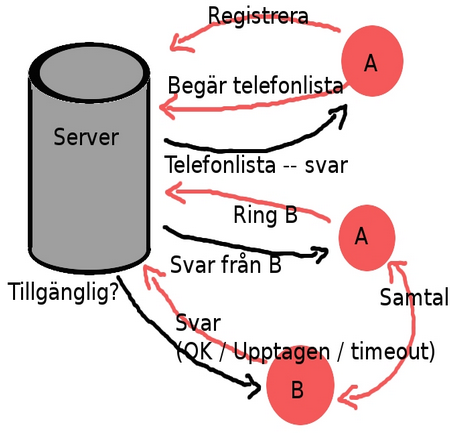
\includegraphics{flowchart.png}}
\caption{This is the pre-project design of Vojpeh (in Swedish). The final design much follows the flow chart, except that Vojpeh does not implement any time-out functionality. The unregistration process is not in the figure.}
\label{micro}
\end{figure}

\section{User manual}
Here follows a step-by-step guide on how to get Vojpeh up and running.
\subsection*{Server}
To start the server run the command \code{java \-jar vojpeh\_server.jar} from the command line. The server is now ready to accept connections from users. To close the server write ''kill'' and press enter in the console.

\subsection*{Client}
\subsubsection*{Setup}
\begin{enumerate}
\item Run the command \code{java -jar vojpeh.jar} from the command line.
\item Press the connect button in the window that pops up.
\item Enter the user name of your choosing.
\item Enter hostname:port in the next window. If left empty standard host and port will be used (localhost:45000).
\item If no problems occured you should now be connected to the server! (This can be confirmed by looking at the previously named ''Connect''-button, it should now display ''Disconnect''. Your user name is also shown to the top left if connected)
\end{enumerate}
\subsubsection*{Calling}
First connect to the server as shown in the Setup part of the user guide. To make a call to another user you double click that users name in the list in the user interface. If done correctly a new window will pop up that shows which user you are trying to call. If the other user doesn’t wish to speak with you, a window will pop up and display that and you will be returned to the start window. If the other user accepts the window will change so that only the other user name is shown. When a call is in progress you can mute your microphone by pressing the mute button. To unmute it, press the button again. To end a call, press the end call button and the call will terminate. This will return you to the start window.
\subsubsection*{Ports}
For the application to function correctly it must be able to accept incoming connections. This goes for both the server and the client. The server uses port 45000 and the client uses ports 45001 and 45002. If the server or client are located on a local network, extra routing may be required for the application to work.

\section{Evaluation}
All requirements except \#6 above are implemented. These were not implemented due to lack of time. There is no nature of the Vojpeh systems structure that would disallow such extensions, but the current implementation would not be difficult to improve with the mentioned functionality. Group calls would possibly need its own \code{MessageType} signal, and be handled separately from other types of calls.

The task is well made. It is nice to get free hands to conduct a project like this one without any guidelines as it inspires programmatic creativity and allows for us to exercise all programming patterns and techniques we have learned so far. As a network communcation task, it might be a bit simple, as the Java language provides so many classes and so much abstracted functionality via its public API that the ''real'' work becomes simply invoking methods on classes written by professionals.

\section{Program code}
In the project, we have used Google Code Subversion as tool for version control. The project exist on Google’s servers at \url{http://code.google.com/p/simple-voip-project/}, where it is open for anyone to checkout the project.




\end{document}
